En esta parte de la investigación se presentan algunos antecedentes relacionados a la detección y pre-diagnóstico de nódulos en distintos órganos y a través de diversas metodologías. Estos ayudarán a entender el enfoque y obtener bases para un correcto desarrollo del proyecto en cuestión.

% Primer antecedente : Segmentation of Skin Lesions Using Convolutional Neural Networks

La investigación de Firdaus et al.\ \cite{firdaus2023} presenta un sistema de segmentación de lesiones cutáneas basado en redes neuronales convolucionales (CNN), utilizando específicamente la arquitectura U-Net, ampliamente reconocida en la segmentación de imágenes biomédicas. Este enfoque busca abordar los desafíos inherentes al análisis de imágenes de dermatoscopia, donde las características de las lesiones cutáneas, como bordes borrosos, variaciones en el contraste, y residuos (cabello y marcadores de regla), dificultan la segmentación precisa y la posterior detección de patologías.

La segmentación precisa de lesiones cutáneas es crucial para el diagnóstico temprano de enfermedades como el melanoma, un tipo de cáncer de piel con alta mortalidad. El estudio emplea el conjunto de datos HAM10000, que contiene más de 10,000 imágenes de dermatoscopia, cubriendo siete categorías diagnósticas de lesiones cutáneas. Estas imágenes, recopiladas en múltiples ubicaciones a lo largo de 20 años, representan una amplia variedad de casos, lo que fortalece la robustez y aplicabilidad del modelo.

El modelo U-Net propuesto se optimizó mediante técnicas de preprocesamiento de imágenes, tales como redimensionamiento, escalado de características, y aumentación de datos, con el objetivo de mejorar la capacidad de generalización y reducir el riesgo de sobreajuste. Durante el entrenamiento, se experimentó con diferentes combinaciones de hiperparámetros, como funciones de pérdida (entropía cruzada binaria y coeficiente de Dice), tasas de aprendizaje y tamaños de lotes. El modelo final alcanzó resultados sobresalientes, con una precisión de píxeles del 95.89\%, un índice de intersección sobre unión (IoU) de 90.37\%, y una puntuación F1 de 92.54\%, lo que evidencia su efectividad y precisión en la segmentación de lesiones.

En comparación con otros métodos de segmentación previos, como campos aleatorios de Markov, bosques aleatorios y máquinas de soporte vectorial (SVM), el modelo U-Net superó a estos enfoques al no requerir extracción de características manual y al ofrecer una segmentación más precisa. La arquitectura U-Net, diseñada con capas de convolución y pooling, permite capturar características complejas de las lesiones, logrando una segmentación de alta calidad que puede ser fundamental para la detección temprana y precisa de enfermedades cutáneas.

En conclusión, el modelo U-Net desarrollado por Firdaus et al.\ demuestra ser una herramienta eficaz para la segmentación de lesiones cutáneas en imágenes de dermatoscopia. Aunque el estudio reconoce limitaciones en términos de recursos computacionales y la necesidad de ajuste fino de hiperparámetros, plantea futuras mejoras que podrían optimizar aún más la segmentación automática de imágenes médicas \cite{firdaus2023}.

\begin{table}[h!]
    \centering
    \begin{tabular}{lccc}
        \toprule
        \textbf{Model} & \textbf{Pixel Accuracy} & \textbf{IoU} & \textbf{F1 Score} \\
        \midrule
        Model 1 & 95.86 & 90.29 & 92.53 \\
        Model 2 & 95.20 & 88.82 & 90.94 \\
        Model 3 & 95.61 & 89.70 & 91.73 \\
        Model 4 & 95.67 & 89.79 & 92.10 \\
        Model 5 & 95.62 & 89.72 & 92.06 \\
        Model 6 & 95.89 & 90.37 & 92.54 \\
        \bottomrule
    \end{tabular}
    \caption{Comparación de Modelos: Precisión de Píxeles, IoU y Puntuación F1}
    \label{tab:comparison}
\end{table}

Además se realizó una comparación con otras investigaciones relevantes y se obtuvieron los siquientes resultados.

\begin{table}[h!]
    \centering
    \begin{tabular}{llccccc}
        \toprule
        \textbf{Research} & \textbf{Method} & \textbf{Dataset} & \textbf{Acc} & \textbf{IoU} & \textbf{F1 Score} \\
        \midrule
        Salih \& Viriri \cite{Salih2020} & SRM+MRF & ISIC 2018 & 0.92 & 0.79 & 0.88 \\
        Jin et al.\ \cite{Jin2021} & CKDNet & ISIC 2018 & 0.93 & 0.79 & 0.87 \\
        Arora et al.\ \cite{Arora2021} & Attn\_U-Net+GN & ISIC 2018 & 0.95 & 0.83 & 0.91 \\
        Proposed* & U-Net & ISIC 2018 & 0.95 & 0.90 & 0.92 \\
        \bottomrule
    \end{tabular}
    \caption{Comparación de diferentes métodos de segmentación de lesiones cutáneas en el conjunto de datos ISIC 2018.}
    \label{tab:comparison_methods}
\end{table}

%% Segunda antecedente : Deep-Learning-Based Morphological Feature Segmentation for Facial Skin Image Analysis

El estudio \citetitle{yoon2023}, donde \cite{yoon2023} proponen un modelo de segmentación de características morfológicas de la piel facial, específicamente arrugas y poros, mediante técnicas de aprendizaje profundo. Este enfoque es relevante para la dermatología estética y el cuidado de la piel, ya que permite realizar análisis detallados de la piel y personalizar recomendaciones de productos cosméticos.

El modelo está basado en la arquitectura U-Net, que ha demostrado ser efectiva en la segmentación de imágenes biomédicas. En este trabajo, U-Net se complementa con mecanismos de atención que mejoran el enfoque en zonas clave, como las áreas faciales donde arrugas y poros son más frecuentes. Además, se implementa una técnica de codificación posicional que aprovecha la disposición típica de estas características en el rostro, mejorando así la precisión del modelo al reducir los falsos positivos y centrarse en las regiones de interés.

Para optimizar la precisión de la segmentación, se desarrolla un método de generación de “ground truth” (GT) adaptado a la naturaleza específica de las arrugas y poros. Este GT se obtiene utilizando mapas de textura específicos: un filtro de alta frecuencia que realza los detalles de las arrugas y un método de pirámide laplaciana para destacar los poros. El conjunto de datos incluyó 314 imágenes faciales obtenidas mediante dispositivos de diagnóstico dermatológico, de las cuales 264 fueron empleadas para entrenamiento y 50 para validación. Las imágenes fueron preprocesadas y anotadas manualmente por especialistas.

Los resultados obtenidos demostraron que el modelo propuesto superó a otros métodos tradicionales de procesamiento de imágenes y arquitecturas de aprendizaje profundo, como U-Net++. Específicamente, el modelo alcanzó un valor de Intersección sobre Unión (IoU) de 0.2341 para arrugas y de 0.4032 para poros, superando los valores de 0.2160 y 0.3669 obtenidos con U-Net++ en estas mismas categorías. En términos de precisión de píxeles, el modelo alcanzó un 95.89%, mientras que la puntuación F1 fue de 92.54%, lo que indica un rendimiento robusto en condiciones variadas de iluminación y textura de la piel.

\cite{yoon2023} concluyen que la integración de mecanismos de atención y codificación posicional en la arquitectura U-Net proporciona una segmentación más precisa de arrugas y poros, con potencial de aplicación en tareas avanzadas como la estimación de la edad de la piel y el análisis de su elasticidad y rugosidad. Este enfoque innovador podría facilitar diagnósticos estéticos y médicos de la piel, permitiendo mejorar la personalización en el cuidado cutáneo \cite{yoon2023}.


\begin{table}[h!]
    \centering
    \caption{Performance Metrics of Different Models}
    \renewcommand{\arraystretch}{1.2} % Adjust row spacing
    \setlength{\tabcolsep}{5pt} % Adjust column spacing
    \begin{tabularx}{\textwidth}{@{}X c c c c@{}}
        \toprule
        \textbf{Models} & \textbf{\#Params} & \textbf{Loss} & \textbf{IoU of Wrinkle} & \textbf{IoU of Pore} \\ \midrule
        U-Net & 17.3 M & 1.243 & 0.2078 & 0.3601 \\
        Reduced U-Net & 4.3 M & 1.250 & 0.2147 & 0.3646 \\
        Reduced U-Net, Attentions & 5.2 M & 1.242 & 0.2250 & 0.3714 \\
        Reduced U-Net, Attentions, Zero-padding (Proposed) & 5.2 M & 1.145 & 0.2341 & 0.4032 \\ 
        \bottomrule
    \end{tabularx}
    \label{tab:models_performance}
\end{table}


%% Tercer antecedente : Skin lesion segmentation method for dermoscopic images with convolutional neural networks and semantic segmentation

El artículo \citetitle{Thanh2021} de \cite{Thanh2021} presenta un método avanzado de segmentación de lesiones cutáneas en imágenes dermoscópicas, diseñado para facilitar la detección temprana de melanoma. Esta técnica utiliza la arquitectura U-Net en combinación con el codificador VGG-16, mejorando la segmentación en áreas de baja intensidad, un aspecto crítico en las imágenes dermoscópicas. El método propuesto es notablemente eficaz en sistemas de cómputo con recursos limitados, como los que carecen de GPU potentes, y ofrece una precisión superior al 95\% tras el entrenamiento. El estudio emplea el conjunto de datos ISIC para evaluar su rendimiento, aplicando métricas de similitud Sorensen-Dice y Jaccard. Los resultados experimentales demuestran que esta técnica supera a otros enfoques basados en redes profundas, especialmente en la segmentación precisa de regiones de baja intensidad en las imágenes.

El enfoque presentado evita la necesidad de preprocesamiento de la imagen, como la eliminación de cabello, la extracción de regiones de interés (ROI) o la mejora del contraste. Este método permite el procesamiento directo de imágenes en color sin la conversión a escala de grises ni la segmentación en canales separados. La implementación de este método se realizó en MATLAB, logrando buenos resultados en términos de sensibilidad y especificidad, con valores promedio de 0.92 y 0.86 para las métricas Dice y Jaccard, respectivamente, en las imágenes de prueba.


%% Cuarto antecedente :  High Performing Facial Skin Problem Diagnosis with Enhanced Mask R-CNN and Super Resolution GAN

En el artículo \citetitle{Kim2023} de \cite{Kim2023}, se propone un sistema mejorado para el diagnóstico de problemas de piel facial mediante una versión refinada de Mask R-CNN combinada con una red generativa adversarial de superresolución (SR-GAN). La piel facial es un factor crucial en la percepción de la edad, salud y belleza de una persona. Para abordar los desafíos técnicos inherentes al diagnóstico de problemas de piel, como acné, manchas y poros, los autores identifican cinco obstáculos técnicos principales: (1) la detección de problemas de pequeño tamaño, (2) la variabilidad en la apariencia de un mismo problema entre diferentes individuos, (3) la similitud visual entre distintos tipos de problemas, (4) la dificultad para detectar múltiples tipos de problemas en la misma imagen y (5) las segmentaciones erróneas en áreas no faciales.

Para superar estos desafíos, se implementan cinco tácticas que mejoran significativamente el rendimiento. En primer lugar, el modelo Mask R-CNN se optimiza mediante capas de fusión y deconvolución, lo que permite detectar características de pequeño tamaño, como poros y arrugas. En segundo lugar, se emplea un SR-GAN para aumentar la resolución de las imágenes de baja calidad, mejorando la precisión en la detección de problemas pequeños. Tercero, se entrenan modelos de segmentación específicos para cada tipo de problema, lo que optimiza la detección al reducir las interferencias de clases no relacionadas. La cuarta táctica consiste en utilizar modelos de segmentación específicos para cada dirección facial (frontal, lateral izquierda y derecha), ya que la posición y visibilidad de ciertos problemas varía según la orientación del rostro. Finalmente, la quinta táctica emplea un modelo de detección de landmarks faciales para descartar segmentaciones en áreas no faciales, como ojos, cejas y cabello, evitando falsos positivos.

Los resultados experimentales muestran que estas tácticas incrementan el rendimiento diagnóstico en un 32.58\% respecto a los modelos CNN convencionales, alcanzando una precisión de 83.38\%. Este enfoque no solo es preciso, sino que es adecuado para implementarse en dispositivos de bajo costo y en aplicaciones móviles, proporcionando una alternativa económica a las visitas clínicas. Los autores sugieren que este sistema podría ser de utilidad en clínicas de cuidado de la piel o como una herramienta accesible para el diagnóstico domiciliario.

\begin{figure}[!ht]
	\begin{center}
		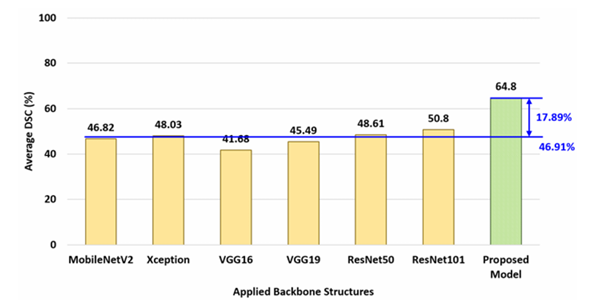
\includegraphics[width=1\textwidth]{2/figures/resultados de cuarto anteedente.png}
		\caption[Comparación del modelo propuesto con otros 6 modelos de redes neuronales]{Comparación del modelo propuesto con otros 6 modelos de redes neuronales.\\
			Fuente: \cite{Kim2023}. \citetitle{Kim2023}. (p. 8)}
		\label{2:fig1}
	\end{center}
\end{figure}


%% Quinto antecedente: 
El artículo titulado \citetitle{Zhong2024} de \cite{Zhong2024} presenta un enfoque innovador para la detección de arrugas faciales, abordando las limitaciones de métodos tradicionales que se ven afectados por interferencias con otras características faciales. Para mejorar la precisión, los autores proponen el uso del modelo DeepLabV3+ junto con una estrategia de etiquetado semi-automática, lo que permite generar datos de entrenamiento más representativos y mejorar la segmentación de arrugas.
La investigación, como podemos ver en las Figuras \ref{2:fig2} y \ref{2:fig3}, emplea técnicas avanzadas como DeepLabV3+, una red optimizada para segmentación de imágenes, y MobileNetV2 para reducir la carga computacional. Además, se desarrolla una estrategia de etiquetado semi-automática combinando anotaciones dermatológicas con mapas de textura generados mediante filtros Wiener y umbralización adaptativa. La precisión del modelo se evalúa mediante el Índice de Similitud Jaccard (JSI).

\begin{figure}[!ht]
	\begin{center}
		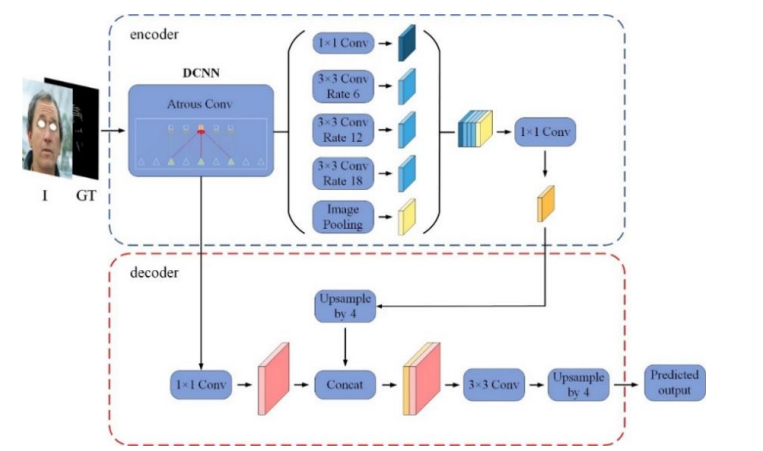
\includegraphics[width=1\textwidth]{2/figures/Meto1.png}
		\caption[Estructura de red de DeepLabV3+]{Estructura de red de DeepLabV3+.\\
			Fuente: \cite{Zhong2024}. \citetitle{Zhong2024}. (p. 4)}
		\label{2:fig3}
	\end{center}
\end{figure}


\begin{figure}[!ht]
	\begin{center}
		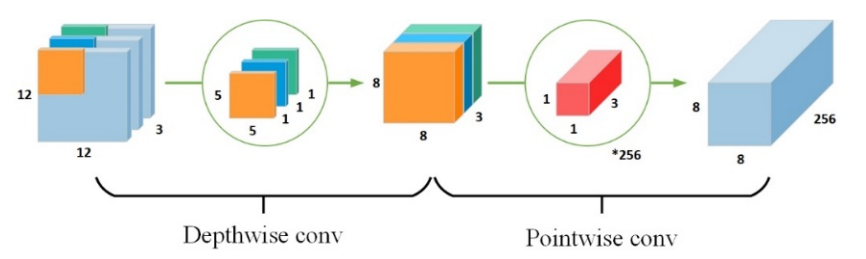
\includegraphics[width=0.80\textwidth]{2/figures/Meto2.png}
		\caption[El proceso de convolución separable en profundidad]{El proceso de convolución separable en profundidad.\\
			Fuente: \cite{Zhong2024}. \citetitle{Zhong2024}. (p. 4)}
		\label{2:fig4}
	\end{center}
\end{figure}


El conjunto de datos se construyó con 300 imágenes de Flickr-Face-HQ, divididas en entrenamiento (225), validación (25) y pruebas (50). Las pruebas se realizaron en un sistema con hardware de alto rendimiento (Intel Core i9-12900K, GPU RTX 3070 y 32GB RAM) y utilizando PyTorch como framework principal.

Los resultados demostraron que el método propuesto supera a enfoques tradicionales como el filtro Hessiano y el modelo U-Net, obteniendo mayores valores de JSI en la frente (0.62) y área ocular (0.64). Además, redujo la cantidad de falsos positivos y mejoró la segmentación de bordes, logrando un mejor desempeño en la detección de arrugas finas.


En conclusión, el modelo DeepLabV3+ con etiquetado semi-automático se mostró más efectivo en la detección de arrugas faciales. Sin embargo, aún enfrenta desafíos en la diferenciación de arrugas muy finas y cabellos, lo que sugiere la necesidad de mejoras futuras para incrementar la precisión del sistema.


%% Sexto antecedente: 

En el artículo de \cite{karshiev2020improved} llamado \citetitle{karshiev2020improved} analiza el problema de la segmentación de lesiones cutáneas, una tarea fundamental para el diagnóstico temprano del melanoma. Aunque el modelo U-Net ha sido ampliamente utilizado en segmentación médica, presenta limitaciones como ralentización en el entrenamiento y problemas con la función de activación ReLU. Para mejorar su desempeño, los autores proponen una versión optimizada que incorpora interpolación bilineal para el upsampling y la función de activación PReLU, lo que mejora la precisión y evita problemas como el sobreajuste.

La investigación emplea un diagrama el cual se puede ver en la Figura \ref{2:fig5} y a su vez varias técnicas clave: la interpolación bilineal sustituye la deconvolución tradicional para mejorar la segmentación de bordes, la función PReLU reemplaza ReLU para prevenir "neuronas muertas" y optimizar la convergencia, y el dropout se utiliza después de cada bloque convolucional para reducir el sobreajuste. Estas modificaciones permiten mejorar la estabilidad y eficiencia del entrenamiento.

\begin{figure}[!ht]
	\begin{center}
		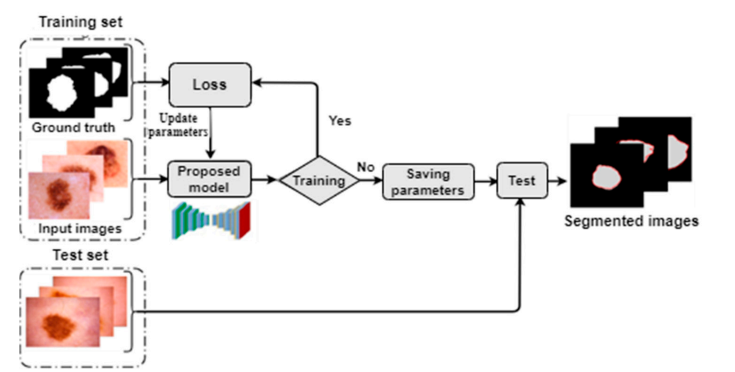
\includegraphics[width=0.80\textwidth]{2/figures/flowchart.png}
		\caption[Diagrama de flujo del sistema propuesto]{Diagrama de flujo del sistema propuesto.\\
			Fuente: \cite{karshiev2020improved}. \citetitle{karshiev2020improved}. (p. 4)}
		\label{2:fig5}
	\end{center}
\end{figure}

El modelo propuesto como se ve en la Figura \ref{2:fig6}, se basa en una arquitectura U-Net modificada con capas convolucionales optimizadas, PReLU, dropout y upsampling mediante interpolación bilineal. Fue entrenado en un sistema con un procesador Intel Core i7-9700K, 32 GB de RAM y una GPU NVIDIA GeForce RTX 2060 SUPER, garantizando un entorno adecuado para el procesamiento intensivo de imágenes médicas.

\begin{figure}[!ht]
	\begin{center}
		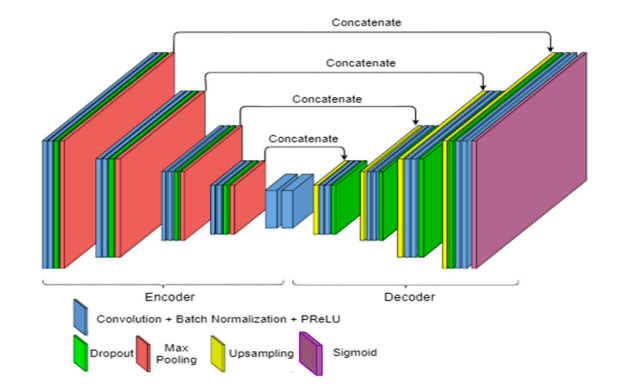
\includegraphics[width=0.80\textwidth]{2/figures/segmentation1.png}
		\caption[Modelo totalmente convolucional propuesto para la segmentación de lesiones cutáneas]{Modelo totalmente convolucional propuesto para la segmentación de lesiones cutáneas.\\
			Fuente: \cite{karshiev2020improved}. \citetitle{karshiev2020improved}. (p. 4)}
		\label{2:fig6}
	\end{center}
\end{figure}

Para el entrenamiento y prueba del modelo se utilizó un conjunto de datos de imágenes dermoscópicas, con 2594 imágenes etiquetadas para entrenamiento y 1000 para prueba. Todas las imágenes fueron preprocesadas, redimensionadas a 256×256 píxeles y convertidas a escala de grises, lo que facilitó la normalización y mejoró la eficiencia del modelo.

Los resultados muestran un alto rendimiento del modelo mejorado, alcanzando una precisión por píxel del 94\% y un coeficiente Dice del 88\%. Estas mejoras permiten reducir artefactos en la segmentación y aumentar la eficiencia computacional en comparación con la U-Net estándar, consolidándose como una alternativa más precisa y robusta para la segmentación de lesiones cutáneas.

En conclusión, la versión mejorada de U-Net supera las limitaciones del modelo original al abordar problemas como gradientes débiles y artefactos en la segmentación. La integración de interpolación bilineal, PReLU y dropout permite lograr una mayor precisión y eficiencia, posicionando este enfoque como una herramienta prometedora para la segmentación de imágenes médicas en el ámbito dermatológico.

%% Séptimo antecedente: 

El artículo titulado \citetitle{Bekmirzaev2021} de los autores \cite{Bekmirzaev2021}, presenta una novedosa técnica de aprendizaje "objeto por objeto" para detectar 11 tipos de lesiones cutáneas faciales mediante segmentación semántica. Los autores destacan que muchas clases de lesiones, como arrugas y manchas, presentan relaciones visuales concurrentes, y explotan esta característica para abordar ambigüedades en la apariencia de las imágenes, mejorando así la precisión en el diagnóstico automatizado.  

Entre las técnicas utilizadas, introducen los módulos REthinker, formados por capas convLSTM/Conv3D locales y un módulo SE como mecanismo de atención. Además, integran estos bloques en redes CNN estándar, junto con técnicas avanzadas como convolución atrous, agrupación espacial piramidal y convolución separable en profundidad, lo que permite una representación más rica y contextual de las lesiones cutáneas.  

La metodología como se observa en la Figura \ref{2:fig7}, se basa en modelar explícitamente las relaciones contextuales entre clases de objetos mediante el aprendizaje "objeto por objeto". Los módulos REthinker se diseñan para mejorar la sensibilidad de la red tanto en contextos locales como globales. Las CNN se modifican para incorporar estos módulos, y los modelos resultantes se entrenan y validan sobre datos dermatológicos cuidadosamente anotados.  

\begin{figure}[!ht]
	\begin{center}
		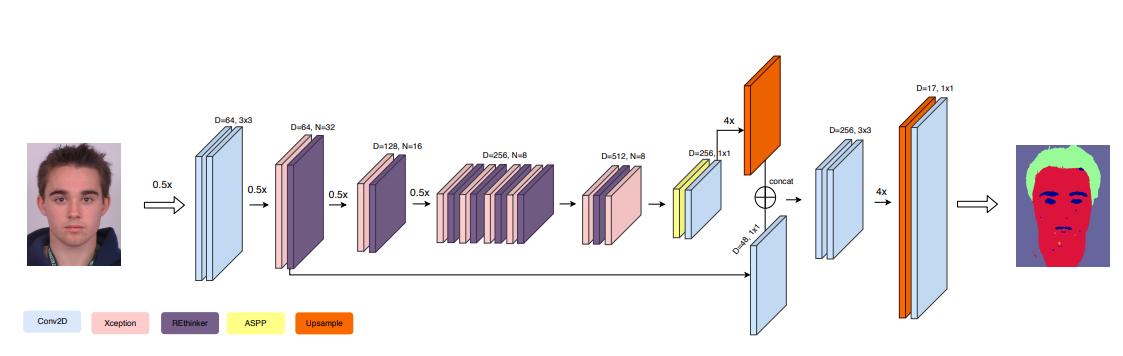
\includegraphics[width=1\textwidth]{2/figures/propose7.png}
		\caption[Propuesta basada en RethNet RE-Xception y el decodificador de DeepLabv3+]{Propuesta basada en RethNet RE-Xception y el decodificador de DeepLabv3+.\\
			Fuente: \cite{Bekmirzaev2021}. \citetitle{Bekmirzaev2021}. (p. 5)}
		\label{2:fig7}
	\end{center}
\end{figure}

Para validar su enfoque, los autores construyen la base de datos propia **MSLD**, que contiene 27,790 imágenes faciales, de las cuales 412 están anotadas con 11 tipos de lesiones cutáneas y 6 clases adicionales. También evalúan sus modelos con el conjunto de datos ISIC 2018, ampliamente utilizado en tareas de segmentación dermatológica.  

Los resultados muestran que su método supera en un 15.34\% en MIoU a redes de segmentación de última generación en el conjunto de datos MSLD, y obtiene buenos resultados en ISIC 2018, lo que demuestra su eficacia en contextos diversos.  

En conclusión, el enfoque propuesto basado en aprendizaje "objeto por objeto" y los módulos REthinker permiten capturar eficazmente relaciones contextuales entre diferentes tipos de lesiones. Esta estrategia mejora considerablemente la precisión de los sistemas de segmentación facial, destacándose como una alternativa poderosa frente a los métodos convencionales.

%% Octavo antecedente:
\cite{Tamilkodi2024} elaboraron el artículo titulado \citetitle{Tamilkodi2024}, que presenta un software avanzado para el análisis de la piel facial que permite identificar características clave como arrugas, poros, manchas y textura, además de predecir edad y género. El sistema compara los resultados con datos de personas del mismo grupo etario, clasifica el tono de piel, genera máscaras visuales para resaltar zonas específicas del rostro y ofrece recomendaciones personalizadas. El objetivo central es desarrollar un modelo robusto capaz de realizar un análisis facial completo en diversos contextos.  

Para lograrlo, el software utiliza redes neuronales convolucionales profundas (D-CNN), apoyadas por modelos preentrenados para la detección de edad y género. También emplea técnicas como KMeans para clasificar el tono de piel y gradientes de Sobel para identificar arrugas. Estas herramientas se integran para ofrecer un análisis visual y cuantitativo de cada característica facial.  

La metodología del sistema incluye la captura de imágenes faciales desde múltiples ángulos, el preprocesamiento mediante técnicas como desenfoque gaussiano y conversión de formatos, seguido del análisis específico de textura, tono y arrugas. Finalmente, los resultados se visualizan en gráficos y máscaras y se utilizan para generar recomendaciones personalizadas para el usuario.  

Como base de datos, se empleó la **Indian Face Age Database (IFAD)**, compuesta por 3,296 imágenes de 55 personas con diversidad de edad, poses, expresiones e iluminación. Esta variedad permite entrenar modelos con mayor capacidad de generalización y robustez en escenarios reales de análisis facial.  

Los resultados como se pueden ver en las Figuras \ref{2:fig8}, \ref{2:fig9} y \ref{2:fig10} ,muestran una alta precisión en la detección de características faciales y predicciones fiables de edad y género. Además, el sistema logra una visualización efectiva mediante gráficos y máscaras que resaltan áreas clave del rostro, lo que mejora la comprensión de los resultados.  

\begin{figure}[!ht]
	\begin{center}
		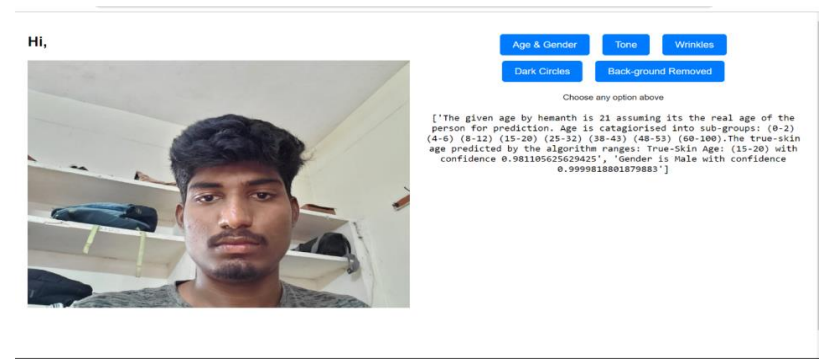
\includegraphics[width=1\textwidth]{2/figures/softres1.png}
		\caption[Detección de edad y género]{Detección de edad y género.\\
			Fuente: \cite{Tamilkodi2024}. \citetitle{Tamilkodi2024}. (p. 6)}
		\label{2:fig8}
	\end{center}
\end{figure}

\begin{figure}[!ht]
	\begin{center}
		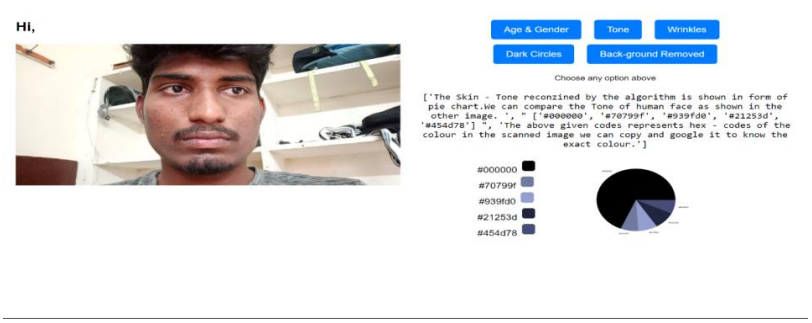
\includegraphics[width=1\textwidth]{2/figures/softres2.png}
		\caption[Análisis del tono de piel]{Análisis del tono de piel.\\
			Fuente: \cite{Tamilkodi2024}. \citetitle{Tamilkodi2024}. (p. 6)}
		\label{2:fig9}
	\end{center}
\end{figure}

\begin{figure}[!ht]
	\begin{center}
		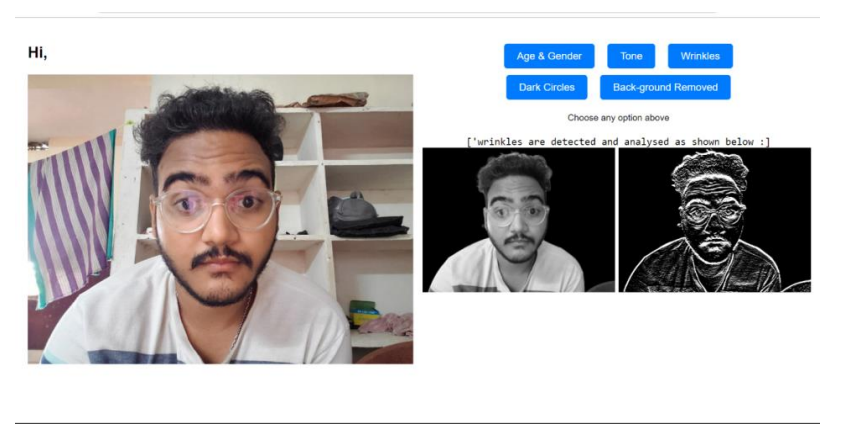
\includegraphics[width=1\textwidth]{2/figures/softres3.png}
		\caption[Análisis de arrugas]{Análisis de arrugas.\\
			Fuente: \cite{Tamilkodi2024}. \citetitle{Tamilkodi2024}. (p. 6)}
		\label{2:fig10}
	\end{center}
\end{figure}

En conclusión, el enfoque propuesto demuestra ser eficaz para detectar estructuras faciales importantes incluso en condiciones variables. Aunque aún no alcanza una precisión perfecta, se reconoce el valor de expandir el conjunto de datos para mejorar el rendimiento. Este modelo tiene un gran potencial para aplicaciones automatizadas en análisis dermatológico y cuidado personalizado de la piel.

%% Noveno antecedente:
El artículo de \cite{moon2024dermatology} llamado \citetitle{moon2024dermatology} se enfoca en la detección automática de arrugas faciales, un tema relevante en dermatología estética, debido a que los métodos manuales de segmentación son subjetivos, costosos y laboriosos. Para abordar este problema, los autores desarrollan un enfoque basado en aprendizaje profundo que incluye la creación del primer conjunto de datos público especializado en segmentación de arrugas (FFHQ-Wrinkle), y una estrategia de entrenamiento en dos etapas que combina un preentrenamiento débilmente supervisado con un ajuste fino supervisado, optimizando así el rendimiento del modelo con un uso eficiente de los recursos de etiquetado.

Se aplican dos enfoques complementarios: primero, un preentrenamiento débilmente supervisado que genera automáticamente mapas de textura mediante filtros Gaussianos sobre 50,000 imágenes no etiquetadas; y segundo, un ajuste fino supervisado que utiliza 1,000 imágenes con máscaras de arrugas anotadas manualmente por expertos. Para la segmentación se emplean arquitecturas de redes neuronales como U-Net y Swin UNETR, que permiten capturar tanto características locales como globales de las arrugas faciales.

La metodología, como podemos ver en la Figura \ref{2:fig11}, consiste en generar etiquetas débiles mediante mapas de textura derivados de imágenes faciales, eliminando regiones no relevantes con un modelo de segmentación facial (BiSeNet). Luego, tres expertos generan manualmente máscaras de arrugas en regiones específicas como la frente y las líneas nasolabiales. El modelo se entrena en dos etapas: primero aprende a predecir texturas con pérdida MSE y luego realiza un ajuste fino con datos manualmente etiquetados y los mapas de textura como entrada adicional, fortaleciendo así su capacidad de generalización.

\begin{figure}[!ht]
	\begin{center}
		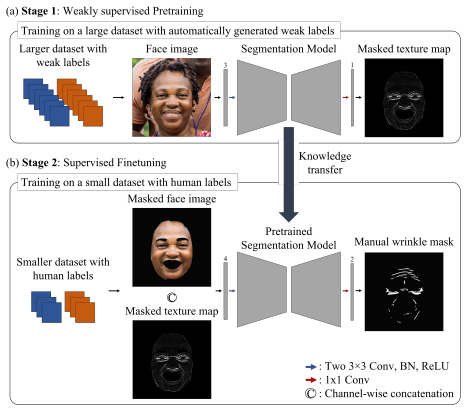
\includegraphics[width=1\textwidth]{2/figures/metoart9.png}
		\caption[Entrenamiento en dos etapas para la segmentación de arrugas faciales]{Entrenamiento en dos etapas para la segmentación de arrugas faciales.\\
			Fuente: \cite{moon2024dermatology}. \citetitle{moon2024dermatology}. (p. 3)}
		\label{2:fig11}
	\end{center}
\end{figure}

El estudio introduce el conjunto FFHQ-Wrinkle, derivado del conjunto de datos FFHQ, compuesto por 50,000 imágenes con etiquetas débiles generadas automáticamente y 1,000 imágenes con anotaciones manuales precisas. Este conjunto incluye una amplia variedad de edades, géneros y etnias, lo que contribuye a la robustez del modelo entrenado y favorece su aplicación generalizada en diversos contextos.

Los modelos entrenados mediante la estrategia propuesta lograron un rendimiento superior en comparación con métodos anteriores, tanto en métricas cuantitativas como cualitativas. La combinación de datos etiquetados automáticamente y manualmente permitió reducir significativamente los recursos necesarios para el etiquetado, manteniendo una alta precisión en la segmentación de arrugas faciales, especialmente en regiones clave del rostro.

La investigación demuestra que la combinación de aprendizaje débilmente supervisado con ajuste fino supervisado mejora sustancialmente la segmentación automática de arrugas faciales. Además, el nuevo conjunto de datos FFHQ-Wrinkle representa un aporte valioso al campo, ya que ofrece una base estandarizada y diversa para futuras investigaciones sobre análisis facial automatizado y aplicaciones en dermatología estética.

%% Décimo antecedente: